%defining document class
\documentclass{article}
\usepackage[utf8]{inputenc}
%setting up page layout
\usepackage{lipsum}
\usepackage[margin=1in,left=1in,includefoot]{geometry}

%Inserting package to import picture/images
\usepackage{graphicx}
% allows control of float positions
\usepackage{float} 
%header and footer
\usepackage{fancyhdr}
 
\pagestyle{fancy}
\fancyhf{}
\fancyfoot[L]{Sudip Siwakoti}
\fancyfoot[C]{\#12956936}
\fancyfoot[R]{\thepage}
\renewcommand{\headrulewidth}{0pt}

\parindent=0pt
\parskip=\medskipamount

%start compiling document
\begin{document}
% creating title page
\begin{titlepage}
%defining alingment of content
	\begin{center}
    \line(1,0){475}\\
% defining spacing    
   [2.5mm]
    \huge{\bfseries INSERT TITLE}\\
    \line(1,0){475}\\
    [3mm]
    \textsc{\Large INSERT REPORT TYPE}\\
    [6cm]
    \textsc{\small \\
    [1mm]
    31005-MACHINE LEARNING\\
    \line(1,0){150}\\
    SPRING 2019}\\
    [6.cm]
    \end{center}
% shifting alingment to left    
    \begin{flushleft}
% inserting line    
    \line(1,0){500}\\
    \textsc{\large Sudent Name: Sudip Siwakoti \\Student Number: 12956936\\ Tutorial: 9 \\ Group: 2 }
    \end{flushleft}
    \lipsum[0]
\end{titlepage}
%inserting table of content.
\tableofcontents
% removing page number form table of content
\thispagestyle{empty}
%clearing rest of the page
\cleardoublepage
%resetting page number 
\setcounter{page}{1}

%starting section and labeling section
\section{INTRODUCTION}\label{sec:intor}


Multiple different approaches are used for establishing the weight of an individual ensemble classifiers that contributes to ensemble’s answer and weighting methods, weighted majority voting, performance weighting, distribution summation, Bayesian combination, Naïve Bayes, Entropy weighting, etc are some example of methods used. On this Paper we will be mainly focusing on majority weighting and Naive Bayes methods.
%starting new section
\section{Description of methods}
\subsection{Weighted Majority Voting}\label{SEC:Methods }
The concept of this technique is based on the general hypothesis that if we have evidence that if majority of the classifier are more qualified then these classifiers can further improve the performance. If we consider a hypothesis ht on class $w_j$ as $d_{t,j}$ such that $d_{t,j}$ is either 1 or 0.\\
\\
Mathematically this can be represented as

$$\displaystyle\sum_{t=1}^{T}w_{t}d_{t,J}=\displaystyle\mathop{\max}_{j=1}^{C}\displaystyle\sum_{t=1}^{T}w_{t}d_{t,j}$$
\\
In this method the weight of the classifier is assigned in proportion to the estimated performance of the classifier
\subsection{Naive Bayes}\
The 


%starting new section
\section{Advantages and Disadvantages}
\subsection{Weighted majority Voting}\label{SEC:Enviro}
\\
\\

\subsection{Naive Bayes}\label{sec:Social}


\section{Purposed Method}
\subsection{Expected Response}\label{sec:EXPECTED}


        
\section{Why is Purposed Method Better}\label{conclusion}
\pagebreak
\section{REFRENCES}\label{refrences}
\begin{flushleft}

\hangindent=2em
\hangafter=1    
Dowling, D., Hadgraft, R., Carew, A., Mccarthy, T., Hargreaves, D. \& Baillie, C. 2016,'Sustainable Engineering', Engineering Your Future An Australasian Guide, 3rd edn, Wiley, 42, pp. 115.\linebreak

Paul, E. 2011, 'Environmental sustainability: From environmental valuation to the sustainability gap', Environmental Sustainability: From 
Environmental Valuation to the Sustainability Gap, vol. 35, no. 5, pp. 629-51.\linebreak


Reddy, T. \& Thomson, R. 2015, Environmental, Social and Economic Sustainability: Implications for Actuarial Science, Institute of Actuaries of Australia, Sydney.\linebreak


Sharifah, R.W.A., Zainuddin, A.M., Jiří, J.K. \& Donald, H. 2014, 'Sustainability engineering for the future', Sustainability Engineering for the Future, vol. 71, pp. 1-10.\linebreak


Staniškis, J.K. \& Katiliūtė, E. 2016, 'Complex evaluation of sustainability in engineering education: case \& analysis', Complex Evaluation of Sustainability in Engineering Education: Case \& Analysis, vol. 120, pp. 13-20.\linebreak


Web Finance 2017, Web Finance, commercial, web Finance, Texas, viewed 17 December 2017, \textless http://www.businessdictionary.com/definition/social-sustainability.html \textgreater.

\pagebreak
\end{flushleft}

\section{Appendix 1: Thankyou Email}\label{sec:appendix }
\begin{figure}[h!]
	\centering
    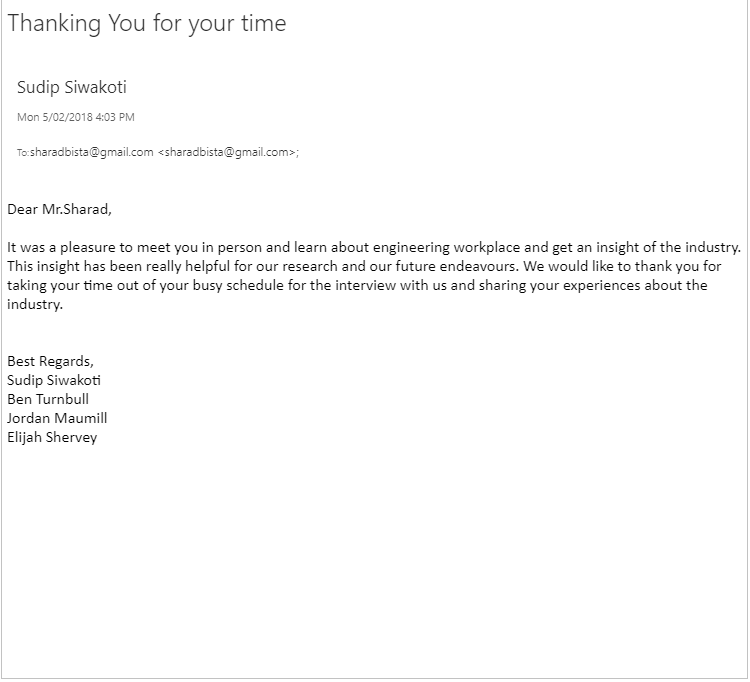
\includegraphics[height= 20cm,width=1\textwidth]{thankyou.PNG}
    \end{figure}
    
\section{Appendix 2: Interview Photo}\label{sec: Questionnaires }
\begin{figure}[h!]
	\centering
    \includegraphics[height= 5cm,width=.5\textwidth]{2.jpg}\linebreak
     
    \centering
    \includegraphics[height= 5cm,width=.5\textwidth]{3.jpg}\linebreak
   
   
    \centering
    \includegraphics[height= 8cm,width=.5\textwidth]{1.jpg}\linebreak
    \end{figure}\pagebreak

\section{Appendix 3: Engineers's Contact Details}\label{sec:APPENDIX3}

\centering
Engineers Name: Sharad Bista.\\
Email: sharadbista@gmail.com\\
Mobile: 0419238101

\end{document}